\documentclass[10pt]{article}
\usepackage[a4paper, tmargin=0.75in, lmargin=0.80in, rmargin=0.80in, bmargin=1in]{geometry}
\usepackage{hyperref}
\usepackage{booktabs}
\usepackage{siunitx}
\usepackage{graphicx}
\usepackage{natbib}
\usepackage{float}
\usepackage{xcolor}
\usepackage{amsmath}
\usepackage{array}
\usepackage{listings}
\usepackage{tikz}
\usetikzlibrary{automata,positioning,arrows.meta}
\usepackage[percent]{overpic}
\pagestyle{plain}

%%%%%%%%%%%%%%%%%%%%%%%%%%%%%%%%%%%%%%%%%%%%%%%%%%
% IMAGE TOGGLE + SNAPSHOT PATH
%%%%%%%%%%%%%%%%%%%%%%%%%%%%%%%%%%%%%%%%%%%%%%%%%%
\newif\ifshowimages
% Out-of-the-box: placeholders compile without PNGs. For final PDF with plots,
% set \showimagestrue (or build with: make without-images toggles \NOIMAGES).
\showimagestrue
\ifdefined\NOIMAGES
  \showimagesfalse
\fi
\graphicspath{{report-draft-1/snapshots/}{figures/}}

%%%%%%%%%%%%%%%%%%%%%%%%%%%%%%%%%%%%%%%%%%%%%%%%%%
% PHAVer / tool listing style
%%%%%%%%%%%%%%%%%%%%%%%%%%%%%%%%%%%%%%%%%%%%%%%%%%
\lstdefinestyle{phaver}{
  basicstyle=\ttfamily\small,
  columns=fullflexible,
  breaklines=true,
  frame=single,
  showstringspaces=false,
  aboveskip=0.5\baselineskip,
  belowskip=0.5\baselineskip,
  literate={_}{{\_}}1
}

\newcommand{\studentname}{Jaideep Khare and Shu-Lin Shih}
\newcommand{\studentnumber}{35193853 and 35199856}
\newcommand{\coursename}{ECE 622: Modeling \& Verification of Embedded Systems}
\newcommand{\semester}{Spring 2026}

\newcommand{\afterprompt}{\par\medskip}

%% Optional width as fraction of \textwidth (default 0.82)
\newcommand{\labfigure}[4][0.82]{%
\begin{figure}[H]
\centering
\ifshowimages
  \includegraphics[width=#1\textwidth]{#2}
\else
  \fbox{\begin{minipage}[c][45mm][c]{0.90\textwidth}
  \centering
  Image omitted in no-image build\\
  \texttt{\detokenize{#2}}
  \end{minipage}}
\fi
\caption{#3}
\label{#4}
\end{figure}
}

\begin{document}

\begin{center}
{\huge{\coursename}} \\
\vspace{2mm}
{\Large{\semester: Lab 3: Hybrid Systems Verification}}\\
\vspace{1mm}
{\Large{Prof. Daniel Holcomb}}
\end{center}

\vspace{5mm}
\hrule
\vspace{1mm}
\hrule

\vspace{3mm}
\begin{tabular}{ll}
Submitted by:   & {\studentname} \\
Student ID:      & {\studentnumber} \\
Lab No.:         & 3 \\
Submission Date: & April 14, 2026 (04/14/26) \\
\end{tabular}

\vspace{3mm}
\hrule
\vspace{1mm}
\hrule

\section*{Overview}
In this lab we used \textbf{PHAVerLite} to compute forward reachable sets of hybrid automata and to check safety-style properties. For each problem we encoded locations with continuous dynamics (written in PHAVer syntax using primed variables, e.g.\ \texttt{x' == v} for $\dot{x}=v$) and discrete jumps with guards/resets, then bounded the analysis using reasonable location invariants. We varied the partition constraint (\texttt{pc}) to study the tradeoff between runtime and precision: smaller \texttt{pc} refines the polyhedral over-approximation and can remove spurious reachability, but increases the number of symbolic locations and CPU time. Throughout, we treated results in the standard soundness direction for over-approximation \citep{Frehse2008STTT}: \textbf{``not reachable''} for a bad set is a proof for the modeled system, whereas \textbf{``reachable''} indicates the property is not proven at that abstraction level and may require refinement. To keep experiments reproducible, long runs were capped with a fixed timeout and recorded as timed-out when necessary.

\section{Part A: Analysis of Bouncing Ball Model}

The bouncing-ball experiment is the canonical hybrid model (continuous flight with gravity, discrete bounce resets). Course notes \texttt{src/module3\_hybrid\_timed.pdf} slides~92--94 illustrate the same formal pattern (locations, flows, guards, resets) used when encoding the ball in PHAVerLite; the lab model instantiates that template for reachability experiments below.

\subsection*{A.1: Reachable sets for two values of \texttt{pc}}
\textit{Use PHAVerLite to compute reachable states with \texttt{pc=0.5} and \texttt{pc=0.05}. Plot both on the same axes (clearly distinguishable). Answer: for each \texttt{pc}, is $(x,v)=(0.55,0.0)$ unreachable based on the plot?}
\afterprompt
\labfigure[0.72]{a1_phaver_graph.png}{A.1: Reachable-state plot used to classify the target $(x,v)=(0.55,0.0)$ at two partition settings.}{fig:a1_overlay}

\noindent We first used the reachable-set plot as a coarse check of whether the target point is plausibly excluded by the reachable enclosure. At the coarser partition (\texttt{pc}=0.5), the enclosure is visibly wider and the target point is not excluded by the plot. After refining to \texttt{pc}=0.05, the enclosure tightens and the target point is visually outside the reachable region.

\noindent For A.1, the plot at \texttt{pc}=0.5 does not let us conclude unreachability of $(0.55,0)$, while the refined plot at \texttt{pc}=0.05 places the point outside the reachable set.

\subsection*{A.2: \texttt{is\_reachable} vs.\ plot; sweep \texttt{pc}}
\textit{Verify $(0.55,0.0)$ with \texttt{is\_reachable} for \texttt{pc=0.5} and \texttt{0.05} (consistency with A.1).}
\textit{Then sweep \texttt{pc} over $0.5$, $0.2$, $0.1$, $0.05$, $0.01$, and $0.005$. If any run exceeds 15 minutes, report time as ``timed out.''}
\afterprompt
Example command form (adjust names to your model):
\begin{lstlisting}[style=phaver]
check = bball.is_reachable(target);
\end{lstlisting}

\begin{table}[H]
\centering
\begin{tabular}{c c c c}
\toprule
Partition \texttt{pc} & Condition reachable? & Num locations reached & CPU time (\si{s}) \\
\midrule
0.5   & yes & 33   & 0.03 \\
0.2   & yes & 71   & 0.077 \\
0.1   & yes & 152  & 0.171 \\
0.05  & no  & 327  & 0.439 \\
0.01  & no  & 2671 & 8.814 \\
0.005 & no  & 5373 & 44.513 \\
\bottomrule
\end{tabular}
\caption{A.2 reachability sweep from PHAVerLite outputs in \texttt{src/lab3.html}.}
\label{tab:a2_pc_sweep}
\end{table}

\noindent\textit{Follow-up (no extra runs).} If you repeated the reachability check for \texttt{pc=1.0}, \texttt{pc=0.075}, and \texttt{pc=0.001}, which case(s) would \emph{definitely} report the target unreachable? Answer from soundness of unreachability under over-approximation and the table above.

\medskip
\noindent The sweep shows the expected precision-runtime tradeoff: as \texttt{pc} decreases, the number of symbolic locations and CPU time increase sharply, but the reachable enclosure becomes tighter. In our runs the reachability verdict flips between \texttt{pc}=0.1 (reachable) and \texttt{pc}=0.05 (not reachable), which is consistent with refinement removing spurious reachability.

\noindent For the follow-up in A.2, among \texttt{pc}=1.0, 0.075, and 0.001, the finest setting \texttt{pc}=0.001 is the one most likely to report the target as unreachable.

\subsection*{A.3: Bounce counter \texttt{n} and peak-height queries}
\textit{Fix \texttt{pc=0.05}. Discuss whether peak height exactly $0.15$ on bounces 1--4 appears consistent with the reachable set plot. Add variable \texttt{n} (init, derivatives per location, resets on jumps). Enforce \texttt{n}$\leq 10$ via an invariant. Add four \texttt{is\_reachable} checks \texttt{n1}\ldots\texttt{n4} for $(x,v)=(0.15,0)$ on each bounce. Submit \texttt{<lastname>\_A3.pha}.}
\afterprompt
\labfigure[0.70]{a3_phaver_graph.jpg}{A.3: Reachable-set plot used to inspect whether $(x,v)=(0.15,0)$ aligns with bounce peaks.}{fig:a3_reachable}
\begin{lstlisting}[style=phaver]
check = bball.is_reachable(n1);
check = bball.is_reachable(n2);
check = bball.is_reachable(n3);
check = bball.is_reachable(n4);
\end{lstlisting}
\labfigure[0.78]{a3_terminal_output.jpg}{A.3: Terminal output for bounce-indexed queries \texttt{n1}--\texttt{n4}.}{fig:a3_terminal}

\noindent In A.3 we used two complementary checks: a geometric inspection of the reachable enclosure to see whether $(0.15,0)$ lies on a plausible peak, and a direct reachability query indexed by bounce count. Both checks point to the same conclusion: the second-bounce peak is consistent with height $0.15$ at zero velocity, while the other peaks do not appear supported at this partition.

\noindent In A.3, both the plot and the bounce-indexed reachability checks indicate that height $0.15$ at zero velocity is consistent with the \textbf{second bounce} at \texttt{pc}=0.05.

\section{Part B: Model of Heating System}

The heating plant is a two-location hybrid: temperature evolves continuously in each mode while a clock \texttt{t} advances at rate one, so time-bounded properties can be expressed as conjunctions involving \texttt{t}. Location invariants (e.g.\ $0\le t\le 10$) keep the reachable set compact for PHAVerLite.

\subsection*{B.1: Reachable set with \texttt{pc=0.3}}
\textit{Encode the heating model in PHAVer syntax. Add a clock \texttt{t} (init 0, derivative 1 in both locations, value retained across jumps). Enforce $0\leq t\leq 10$ in both locations. Plot reachable states: $x$-axis time, $y$-axis temperature.}
\afterprompt
\labfigure[0.80]{b1_phaver_state_graph.png}{B.1: Heating-system reachable set (time on $x$-axis, temperature on $y$-axis) at \texttt{pc=0.3}.}{fig:b1_heating}
\noindent We implemented the clocked hybrid model and plotted the reachable set in the time--temperature plane. The resulting tube provides a compact summary of the system's possible temperature evolution over the bounded horizon, and it makes the effect of switching between modes visible as changes in the reachable enclosure.

\noindent In B.1, we generated the time--temperature reachable set over $t\in[0,10]$ using \texttt{pc}=0.3.

\subsection*{B.2: Time-bounded temperature property}
\textit{From initial \((\text{cool}, t{=}0, x{=}22)\), show temperature goes below \SI{20}{\celsius} within \SI{0.98}{\second}. Use a counterexample region with \texttt{t==0.98} (not \texttt{t>=0.98}). Find the largest \texttt{pc} (within \SI{0.1}{} of the true threshold) for which the bad set is unreachable. Submit \texttt{<lastname>\_B2.pha}.}
\afterprompt
\noindent We expressed the requirement as a bad set at the exact time slice $t=0.98$ and then swept \texttt{pc} to find where the abstraction becomes too coarse to exclude the bad region. In our sweep, the check remained \emph{not reachable} below \texttt{pc}=1.3 and became \emph{reachable} at \texttt{pc}=1.3, giving a tight bracket for the requested threshold.

\begin{lstlisting}[style=phaver]
bad = heatingsystem.{$ & t == 98/100 & x > 20};
check = heatingsystem.is_reachable(bad);
\end{lstlisting}
\noindent In B.2, the largest partition constraint that still reports the bad set as \textbf{not reachable} is \texttt{pc}=1.2; at \texttt{pc}=1.3, the bad set becomes \textbf{reachable}.

\section{Part C: Car Acceleration and Braking}

\noindent\textit{Scenario: two intersections \SI{500}{\meter} apart; stop sign then traffic light. Full stop at sign; accelerate at \SI{3.5}{\meter\per\second\squared}. Braking for red light starts between \SI{250}{\meter} and \SI{300}{\meter} past the stop sign (i.e.\ \SI{200}{\meter}--\SI{250}{\meter} from the light). Braking acceleration \SI{-5.5}{\meter\per\second\squared} until stop.}

The red-light onset is modeled as \textbf{nondeterministic}: the jump from acceleration to braking may occur at any position in $[\SI{250}{\meter},\SI{300}{\meter}]$. The invariant $x\le \SI{300}{\meter}$ in the accel location forces a decision before leaving that window.

\subsection*{C.1: Hybrid automaton diagram}
\textit{Circle locations; label guards on jumps; derivatives of position and velocity per location; location invariants (including to force transitions when guards stay true).}
\afterprompt
\begin{figure}[H]
\centering
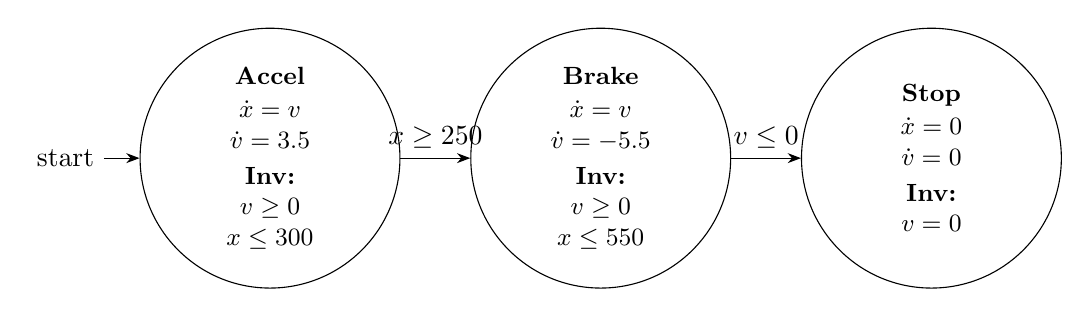
\begin{tikzpicture}[
  ->,
  >=Stealth,
  node distance=4.2cm,
  on grid,
  auto,
  every state/.style={
    draw,
    circle,
    minimum size=3.3cm,
    inner sep=3pt,
    align=center,
    font=\small
  }
]
\node[state, initial] (accel) {\textbf{Accel}\\[1pt]
  $\dot{x}=v$\\
  $\dot{v}=3.5$\\[2pt]
  \textbf{Inv:}\\
  $v\ge 0$\\
  $x\le 300$
};
\node[state] (brake) [right=of accel] {\textbf{Brake}\\[1pt]
  $\dot{x}=v$\\
  $\dot{v}=-5.5$\\[2pt]
  \textbf{Inv:}\\
  $v\ge 0$\\
  $x\le 550$
};
\node[state] (stop) [right=of brake] {\textbf{Stop}\\[1pt]
  $\dot{x}=0$\\
  $\dot{v}=0$\\[2pt]
  \textbf{Inv:}\\
  $v=0$
};
\path (accel) edge node {$x\ge 250$} (brake)
      (brake) edge node {$v\le 0$} (stop);
\end{tikzpicture}\\[0.6em]
\caption{C.1: Hybrid automaton for the car (initial full stop at $x=0$).}
\label{fig:c1_diagram}
\end{figure}

\subsection*{Analytical cross-check (kinematics)}
Uniform acceleration segments satisfy the usual SUVAT relations; they are useful to sanity-check extreme speeds and stopping distances against the reachable set, not as a substitute for PHAVerLite proofs:
\begin{align}
v^2 &= u^2 + 2 a s, \label{eq:suvat1} \\
s &= ut + \tfrac{1}{2} a t^2, \label{eq:suvat2} \\
v &= u + a t. \label{eq:suvat3}
\end{align}
We used these equations to compute simple bounds that explain the reachable envelopes. Starting from rest ($u=0$) with $a=\SI{3.5}{\meter\per\second\squared}$, the speed at the braking window endpoints is:
\[
v(250)=\sqrt{2\cdot 3.5\cdot 250}\approx\SI{41.8}{\meter\per\second},\qquad
v(300)=\sqrt{2\cdot 3.5\cdot 300}\approx\SI{45.8}{\meter\per\second}.
\]
The corresponding times to reach those positions follow from \eqref{eq:suvat2} with $u=0$:
\[
t(250)=\sqrt{\tfrac{2\cdot 250}{3.5}}\approx\SI{11.95}{\second},\qquad
t(300)=\sqrt{\tfrac{2\cdot 300}{3.5}}\approx\SI{13.09}{\second}.
\]
Once braking begins ($a=\SI{-5.5}{\meter\per\second\squared}$), \eqref{eq:suvat3} shows velocity decreases monotonically, so the maximum braking speed is the entry speed at the braking trigger. This is why Property~2 is expected to hold for the concrete dynamics, while Property~3 can fail depending on when braking is triggered (late braking can still enter at speeds above \SI{40}{\meter\per\second}).

\subsection*{C.2: PHAVer model and reachable set}
\textit{Translate to PHAVer. Use reasonable invariants to bound the state space. With \texttt{pc=3.0}, plot reachable states: position ($x$-axis) vs.\ velocity ($y$-axis).}
\afterprompt
\noindent We encoded the car dynamics and red-light nondeterminism in PHAVerLite, bounded the state space with simple invariants, and generated the reachable set at \texttt{pc}=3.0. We then exported the reachable region and plotted position versus velocity to visualize the envelope of possible behaviors under the uncertain braking start.
\begin{figure}[H]
\centering
\begin{overpic}[width=0.85\textwidth]{c2_car_reachable_x_v.jpg}
  \put(50,2){\makebox(0,0){\small Position $x$ (m)}}
  \put(2,50){\rotatebox{90}{\small Velocity $v$ (m/s)}}
\end{overpic}
\caption{C.2: Reachable states in the $(x,v)$ plane at \texttt{pc}=3.0 (export from PHAVerLite), with axis labels for position and velocity.}
\label{fig:c2_reachable}
\end{figure}

\noindent In C.2, we generated the reachable states in the $(x,v)$ plane at \texttt{pc}=3.0, with position on the horizontal axis and velocity on the vertical axis.

\subsection*{C.3: Three reachability properties}
\textit{For each property below, give the exact \texttt{is\_reachable(...)} query, include one screenshot with PHAVerLite text output for all three checks, and explain why unreachability (or the appropriate abstraction argument) proves the property true/false. Submit \texttt{<lastname>\_C3.pha}.}

\begin{table}[H]
\centering
\begin{tabular}{p{0.45\textwidth} c c}
\toprule
Property statement (compact) & \texttt{pc}=3.0 & \texttt{pc}=1.2 \\
\midrule
Stops before the second intersection & not proven & satisfied \\
$v \le \SI{46.5}{\meter\per\second}$ during braking & not proven & satisfied \\
$v \le \SI{40.0}{\meter\per\second}$ during braking & not proven & not proven \\
\bottomrule
\end{tabular}
\caption{C.3 property statements and outcomes at two partition constraints.}
\label{tab:c3_properties}
\end{table}

\medskip
\noindent\textbf{Bad-state queries (submitted \texttt{jkhare\_C3.pha}).} Each property is checked by reachability of a \emph{violation} set; proving the property would require \texttt{not reachable} for that set.
\begin{lstlisting}[style=phaver]
p1_bad = car_sys.{Brake & x >= 500 & v >= 0.001};
p1_bad_reach = car_sys.is_reachable(p1_bad);
p2_bad = car_sys.{Brake & v >= 46.5};
p2_bad_reach = car_sys.is_reachable(p2_bad);
p3_bad = car_sys.{Brake & v >= 40.0};
p3_bad_reach = car_sys.is_reachable(p3_bad);
\end{lstlisting}
\noindent Here \texttt{v >= 0.001} in P1 separates ``still moving'' from a full stop at $v=0$. At \texttt{pc=3.0}, PHAVerLite reported \textbf{reachable} for all three bad sets; therefore \textbf{none} of the three properties is formally proven as stated (unreachability would be required for a sound proof). Reachability here may be due to over-approximation, but it does not establish safety---tighter \texttt{pc} or alternative encodings would be needed to refine the verdict.

\begin{lstlisting}[style=phaver,caption={C.3: PHAVerLite output summary for the three property checks (pc=3.0).},label={fig:c3_output}]
p1_bad is reachable.
p2_bad is reachable.
p3_bad is reachable.
\end{lstlisting}

\noindent To distinguish genuine violations from conservatism, we reran the same C.3 checks with a tighter partition (\texttt{pc}=1.2). In that refined run, PHAVerLite reported Property~1 and Property~2 bad sets as \textbf{not reachable}, while Property~3 remained reachable.

\noindent For Property~2 specifically, the concrete dynamics strongly support the safety claim: the car starts from rest, accelerates at \SI{3.5}{\meter\per\second\squared} for at most \SI{300}{\meter} before braking, so the largest possible entry speed into braking is $v_{\max}=\sqrt{2as}=\sqrt{2\cdot 3.5\cdot 300}\approx\SI{45.8}{\meter\per\second}<\SI{46.5}{\meter\per\second}$, and braking only decreases speed.

\noindent In C.3, the coarse run at \texttt{pc}=3.0 does not prove any of the three claims, while the refined run at \texttt{pc}=1.2 proves Property~1 and Property~2 (bad sets not reachable) but still does not prove Property~3.

\subsection*{C.4 (ECE 622 only): 0--60\,MPH time estimate}
\textit{Add a time variable; \SI{60}{mph} \(=\) \SI{26.8}{\meter\per\second}. Use \texttt{pc=3.0}. Two queries: (i) \SI{26.8}{\meter\per\second} unreachable by time $T$; (ii) reachable by time $T+\SI{0.1}{\second}$. Report an interval for 0--60 time. Submit \texttt{<lastname>\_C4.pha}.}
\afterprompt
A separate automaton \texttt{car\_c4} adds $t$ with $\dot{t}=1$ in the \texttt{Accel} location (constant acceleration from rest, $\dot{v}=3.5$). Bracketing queries at $T=\SI{7.6}{\second}$ and $T+\SI{0.1}{\second}=\SI{7.7}{\second}$:
\begin{lstlisting}[style=phaver]
q_before = car_c4.{Accel & t <= 7.6 & v >= 26.8};
r_before = car_c4.is_reachable(q_before);
q_after  = car_c4.{Accel & t <= 7.7 & v >= 26.8};
r_after  = car_c4.is_reachable(q_after);
\end{lstlisting}
With \texttt{pc=3.0}, the tool reported \texttt{q\_before} not reachable and \texttt{q\_after} reachable, so the 0--60\,mph time lies in the interval \textbf{$(\SI{7.6}{\second},\SI{7.7}{\second}]$} (consistent with $t=v/a$ for constant $a$ at \SI{26.8}{\meter\per\second}).

\noindent In C.4, the model brackets the 0--60\,mph time in the interval \textbf{$(\SI{7.6}{\second},\SI{7.7}{\second}]$}.

\section*{Conclusion}
Across Parts A and B we saw the central practical lesson of PHAVerLite reachability: decreasing \texttt{pc} substantially increases cost (locations and runtime) but can sharpen the reachable enclosure enough to change the reachability verdict for a boundary target. For the heating model, bracketing over \texttt{pc} provided a concrete way to locate where the abstraction stops being strong enough to exclude a time-slice counterexample. In Part C, we encoded environmental uncertainty as nondeterminism in the braking trigger and checked safety-style statements as bad-state reachability queries; the over-approximate semantics make \emph{unreachability} the reliable proof direction. In our runs, the three C.3 bad sets were reachable at \texttt{pc}=3.0 (so not proven), while the C.4 bracketing approach produced a narrow and interpretable 0--60\,mph time interval.

\appendix
\section*{Appendix: Tooling and submission artifacts}
This report template was adapted from the Lab~2 \texttt{latex-build} layout. Build with \texttt{latexmk} (see \texttt{README.md}). PHAVerLite models and plots were produced on the course toolchain; figures can be synced via Git alongside this \texttt{.tex} file.

\textbf{Reproducibility (Part~C).} Scripts under \texttt{lab3/modeling\_car/}: \texttt{run\_c3.sh} (timeout-wrapped PHAVerLite), \texttt{check\_c3\_properties.sh}, \texttt{plot\_c3.sh} for the $(x,v)$ figure; \texttt{lab3/modeling\_car/c4/run\_c4.sh} for C.4 bracketing runs.

\textbf{Files to submit (replace \texttt{<lastname>} per handout):}
\begin{itemize}
\item \texttt{<lastname>\_A3.pha}
\item \texttt{<lastname>\_B2.pha}
\item \texttt{<lastname>\_C3.pha}
\item \texttt{<lastname>\_C4.pha} (ECE~622 only)
\end{itemize}

\bibliographystyle{plainnat}
\bibliography{references}

\end{document}
